\section{Theory of Operations}

\subsection{Introduction}
The \textbf{Gpio} module is configurable with parameters for setting data and address widths. It interfaces with the CPU via the APB3 bus. The signals \textbf{gpioInput}, \textbf{gpioOutput} and \textbf{gpioOutputEnable} are designed to interface with external hardware, such as a tri-state buffer, to facilitate bi-directional communication on physical pins.

\begin{figure}[h]
  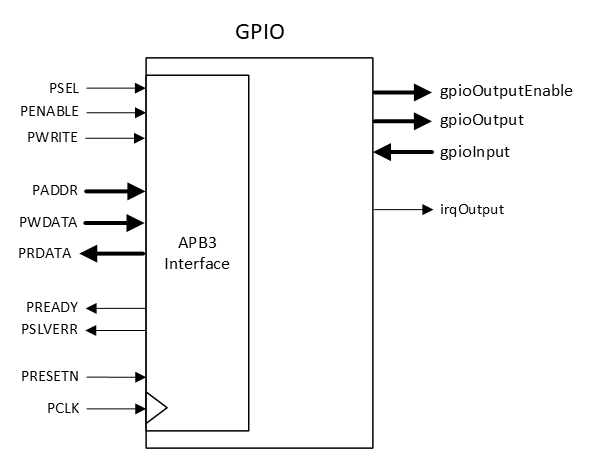
\includegraphics[width=0.90\textwidth]{images/block-diagram-gpio.png}
  \caption{Gpio Block Diagram}\label{fig:block-diagram}
\end{figure}

\newpage
\subsection{Interface Timing}

Gpio has a synchronous APB3 interface, and a Gpio interface. The timing diagram shown below
in Figure~\ref{fig:timing} represents an instantiation with the following
parameters.

\begin{lstlisting}[language=Scala]
val myGpio = new Gpio(
  dataWidth = 16, 
  addrWidth = 16 ) 
\end{lstlisting}

\begin{figure}[h]
  \includegraphics[width=\textwidth]{images/Gpio-timing.png}
  \caption{Timing Diagram}\label{fig:timing}
\end{figure}

This shows the operation of the basic read/write register operations following the APB protocol. Registers DIRECTION, MODE, and OUTPUT are
written to, while register INPUT is read from.

The \textit{gpioOutputEnable} port is driven to a value of 0x000F after 0x000F is written to the DIRECTION register 
at address 0x00. Next, the MODE register at address 0x06 is written a value of 0x0009. The \textit{gpioOutput} port 
then has a value of 0x0009 because of the open-drain mode operation. 

The OUTPUT register is then written a value of 0x0006 at address 0x02. \textit{gpioOutput} takes on a value of 0x000F
since the MSB and LSB are operating on open-drain mode, and the middle two bits are operating on push-pull mode. 

The INPUT register is read from at address 0x04, which has a value of 0x0070 since \textit{gpioInput} has a value fo 0x0070.
On the final transaction, PSLVERR goes high because an invalid address is written to.

